\section{Literature Review} % (fold)
\label{sec:literature_review}

% section literature_review (end)

This section cover the literature review, as well as required background information on Bluetooth and ECG.

\subsection{Electrocardiogram} % (fold)
\label{sub:electrocardiogram}

Most of the reviewed literature discuss or mention ECG in some form or another, because of it's high technical requirements. However, we found many inconsistencies and simplifications about ECG, that in worst case may have invalidated parts of previously conducted research. Because of this, we spent some time understanding both the measurement itself and how it is carried . In the following section we introduce ECG before reviewing other research involving the diagnostic tool.

Electrocardiogram is a measurement of the electrical activity around the heart. The measurements are done by a set of external electrodes attached to the skin at certain places around the chest. These electrodes measure the depolarization of electrical charges that happen in the cell membranes covering the heart at every heart beat. An ECG is conducted by having either 3, 5 or 12 leads. The term lead refers to the voltage difference \textit{between a given pair} of electrodes, parallel to the direction of the lead. Based on the signal strength of each lead, cardiologists can get information about angles and properties of the heart. The leads can either be actual or derived from a vector model\footnote{ The Cabrera circle uses a vector representation to give a good overview of the different leads, and their relationship} based on 2 or more actual leads. Typically 5 electrodes can be used for a 3 and 5-lead ECG, where one of the electrodes are used as a reference point.\footnote{ Also referred to as \emph{ground}.} It is however important to note that the amount of electrodes don't necessary correspond to the number of leads, and the amount of derived leads does not necessary correspond the the number of actual leads. The terminology here seem to confuse a lot of people, as we have seen and heard in both literature and in practice. Alesanco and García are among the few that describe this correctly in \cite{Alesanco:2010kc}, where they state that \textit{``(...) only eight leads should be transmitted since the other four can be derived from them''}. The this confusion is not unfounded, as there exist several techniques for deriving different leads from other leads. As we'll see later, a 12-lead EASI ECG may be derived from 5 electrodes capturing only 3 actual leads (or vectors). Even the traditional 12-lead ECG, is derived from 10 electrodes\footnote{ In a 12-lead ECG the electrodes are placed at each extremity (limb) and 6 on the chest.} which capture 9 actual leads. The differences roles these leads play in practice, are discussed further in Section~\ref{sec:clinical_context}. The consequence of this confusion is that previous research either make incorrect assumptions~\cite{jenniferporcello:2015wv} or report ambiguous results that are hard to verify. Some research \cite{yubin:2012tr, Lee:2009bu, Alesanco:2010kc}, only consider 1 or 2 leads, which has been proven insufficient by~\cite{Drew:1998wp}.

\begin{figure}[H]
\centering
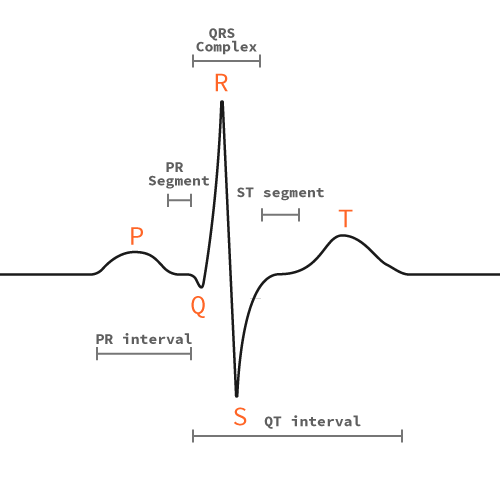
\includegraphics[scale=0.45]{img/figures/QRS.png}
\caption{QRS Complex with interval annotations}
\label{fig:qrsAnnotations}
\end{figure}


\noindent
After the leads are sampled in a wireless ECG solution, they can be streamed in raw, or compressed and optimized for transmission\cite{Balouchestani:2013dr, Alesanco:2010kc}. In order to reduce the scope of this project, we will only focus on the the core aspects of ECG. Different compression and low sampling techniques are therefore omitted completely. After being transmitted, the signals are analyzed at a processing unit, where common angles and intervals in the QRS complex as well as heart rate are calculated. The QRS complex as seen in Figure~\ref{fig:qrsAnnotations} denotes the plot or graphical representation of the electrical signals. On a per lead basis, these plots are printed on gridded paper or displayed on a monitor. Cardiologists learn to analyze the leads and are able to make a diagnosis based on different intervals in the complex, among other things. An overview of some common intervals and the different cardiac diseases they indicate are presented in Table~\ref{tab:characteristicECGintervals}. Based on this analysis, the ECG system may automatically trigger alarms if certain thresholds in the intervals are exceeded.

\begin{table}[]
\centering
\caption{Characteristic ECG intervals from \cite{Jara:2012fi}}
\label{tab:characteristicECGintervals}
\begin{tabular}{|l|l|}
\hline
\textbf{Interval QRS \textgreater 120ms} & \begin{tabular}[c]{@{}l@{}}Ventricular hypertrophy, necrosis, BCRRD,\\ BCRI, pacemakers, cardiomyopathies,  \\ electrolyte abnormalities.\end{tabular}     \\ \hline
\textbf{Interval PQ \textgreater 200ms}  & Frist-degree AV block                                                                                                                                      \\ \hline
\textbf{Interval PR \textless 120ms}     & \begin{tabular}[c]{@{}l@{}}Tachycardia, WPW, manners or \\ headphones low rates.\end{tabular}                                                              \\ \hline
\textbf{Interval QT \textgreater 450ms}  & \begin{tabular}[c]{@{}l@{}}Antiarrhytmic medicines, ischemic heart deisease, \\ cardiomyopathies, hypocalcemia, mixedema, \\ long QT syndrome\end{tabular} \\ \hline
\textbf{Interval QT \textless 350ms}     & \begin{tabular}[c]{@{}l@{}}Hypercalcemia, hyperkalemia,  early \\ repolarization, digoxin\end{tabular}                                                     \\ \hline
\end{tabular}
\end{table}

We have reviewed several earlier projects involving wireless ECG. Below we will assess one such project, while others will be discussed in~\ref{sub:bluetooth}. In Chou and Hibbs 2006 paper \cite{ChulsungPark:2006tf} they present ``An ultra-wearable, wireless low power ECG monitoring system''. They have developed and tested a contact-less ECG capacitive sensor based on insulated bio-electrodes. They imagine that these sensors can integrated into clothes, making ECG monitoring ultra-wearable. They recognize that related work based on either standard wireless interfaces or general purpose sensor nodes suffer from large form factor, low battery lifetime or low transmission speed. Because of this, their approach involve using proprietary and custom hardware in order to reach their goals. Aside from the tiny form factor, an interesting observation is their solution's power consumption, which is less than 10 mA in transmission mode and 22 mA in receiving mode. As we'll see later, this is 10-20 times the average current drawn from today's low energy sensors based on wireless standards like Bluetooth Smart. In terms of ECG, their solution support 1000 Hz sampling rate, and the analog to digital converter (ADC) is configured for 12-bit resolution. They mention their system uses 3 ECG sensors. Assuming they are referring to electrodes, and that one is for \emph{ground}, this means they can only do a 1-lead ECG. Further, they do not address any clinical aspects of their work.

% subsection electrocardiogram (end)

\subsection{Bluetooth and ambulatory ECG} % (fold)
\label{sub:bluetooth}

In accordance with our research goal of assessing available technology, Bluetooth was an attractive technology. This was because of its widespread presence\footnote{ In 2010, Bluetooth SIG estimated an annual sale of 2 billion Bluetooth enabled devices.}, as well as the low energy features introduced with version 4.0 of the specification. Bluetooth was standardized as IEEE 802.15.1, but IEEE no longer maintains the standard. The Bluetooth Special Interest Group (SIG) is comprised of more than 25,000 corporate members, which today maintain and oversees the development of the specification. There are two other IEEE 802.15 standards discussed in relevant literature, namely 802.15.4 and 802.15.6. The first one is likely to play a significant role in the development of future IoT applications.\footnote{ See Google's Thread protocol and Zigbee for implementations of this standard.} As the second one is still in development, this thesis has not assessed the work on 802.15.6. However, of these standards and their implementations, Bluetooth is the most available today. In this section we will cover the basics of Bluetooth Smart and discuss related research projects using the technology in combination with ECG monitoring.

\subsubsection{Bluetooth Smart} % (fold)
\label{ssub:bluetooth}

Bluetooth originated from Ericsson in 1994, and has it's name from a Danish/Norwegian viking king that was characterized as a ``good communicator''. Since it's origin, the standard has seen 4 major releases, and several minor ones.\footnote{ The latest of which (4.2) was released in December 2014} The next big release, version 5.0 is currently being being drafted, and is expected to be formally announced later this year. 

Version 4.0 introduced new low energy features, which was originally branded with the suffix ``LE'' or ``Low Energy''. Because of confusion around the ``low energy'' devices and those implementing older versions of the standard, Bluetooth SIG announced their new branding strategy in 2011. The new logo and name read \textit{Bluetooth Smart}. Throughout this thesis we will focus exclusively on the low energy features of the standard and we believe the suffix ``low energy'' is less ambiguous than ``Smart''. Because of this we will be using both the old and new name based on what's most describing.

% subsubsection bluetooth (end)

\subsubsection{GATT and Profiles} % (fold)
\label{ssub:gatt_and_profiles}

The Bluetooth standard specifies a series of communication protocols that together constitute the complete Bluetooth stack. This stack is separated in two; the \emph{Host} and \emph{Controller}. The controller stack is concerned with the lower network layers and is usually implemented in the firmware of silicon devices containing a Bluetooth radio. The host stack are upper layers, and is usually implemented as part of a operating system and runs on a processor together with the user application. With resource constrained devices such as those we'll investigate in this thesis, both the controller and host can be bundled together. They will then run on the same microprocessor, making up what is known as a ``hostless'' system. See Figure~\ref{fig:bleNordicHost}. 


\begin{figure}[H]
\centering
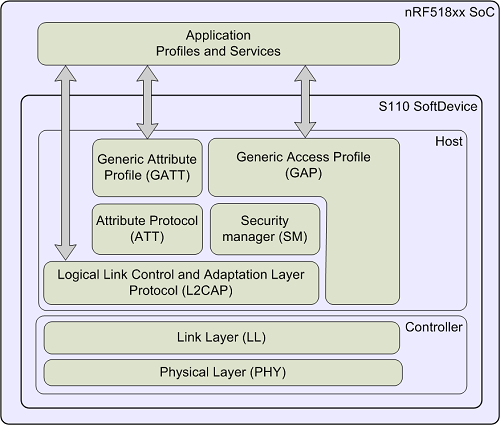
\includegraphics[scale=.8]{img/figures/bleNordicHost.png}
\caption{Overview of the Bluetooth protocol stack on a hostess system~\cite{nordicSDK}}
\label{fig:bleNordicHost}
\end{figure}


% TODO wite about advertising, connection establishment? roles (master and slave / initiator advertisor)

In this thesis we are most concerned with the higher layer protocols, more specifically the GATT profiles. This is an acronym for Generic Attribute Profile, and it is responsible for ensuring interoperability in data exchange between two two Bluetooth devices. The profile defines the types of state data that a device exposes and how that data can be used. Profiles are organized in services, which contain one or more characteristics and descriptors. The profiles and its characteristics are specified by working groups within Bluetooth SIG. The process of how these are developed and implemented are discussed in Section~\ref{sub:interoperability}. More information about how connections are established and data is transmitted, can be found in Section~\ref{ssub:maximum_throughput}.

% subsubsection gatt_and_profiles (end)

\subsubsection{Bluetooth enabled ambulatory ECG} % (fold)
\label{ssub:bluetooth_enabled_ambulatory_ecg}

We have reviewed multiple previous research projects evaluating Bluetooth Low energy as a wireless technology for streaming ECG data. In this section we will review two of them.

Jara et at. evaluated Bluetooth low energy as a technology for streaming continuous data from a wearable ECG in their 2012 paper. Similarly to our project, they focused on analyzing the capabilities of Bluetooth Low Energy as a medium for streaming raw ECG data. Their initial evaluation concluded that it was necessary to compress the ECG signals before transmission. They built a prototype based on a Bluegiga development kit. This development kit comes with its own Bluetooth API, built on top of the Bluetooth stack, which is programmable with a language called BG-script. They do not mention the amount of leads simulated, and their calculations are hard to follow. For their experiments, they operated with a ECG sampling rate of 300 samples/second. We were unable to recompute their calculated throughput, but they conclude that Bluetooth Low Energy in 2012 is not well suited for raw ECG transmission. However, a lot has happened with the specification since then.

Another paper describing ECG data transmission with Bluetooth Low Energy (BLE) is \cite{Anonymous:1SQ78ejy}. They built a three tier of 2 development kits and an Android application. This paper is from 2013, at which time Android did not fully support low energy Bluetooth through their SDK. Because of this, their system is comprised of 3 parts, one low energy board with a Bluetooth interface, one ``converter'' board, that speaks both BLE and Bluetooth 2.1. This board is responsible for proxying the data from the sensor board through to the Android application via Bluetooth 2.1. At the sensor board, they developed a ECG patch system, which records ECG through by using 4 electrodes. They operate with a maximum data rate of 306 kbit/s over the BLE connection, and they claim ECG has to be sampled with at least 250 samples/s. Finally, of interest to this project, they did some preliminary battery tests, and concluded that the batteries lasted between 9 and 13 hours depending on the surrounding temperature.

Other literature related to ECG and its clinical requirements is discussed further in Section~\ref{sub:evaluation}. One common denominator through the review of these and other research projects, is that no one seems to agree on what's the required sampling rate for ECG, and the size of each sample should be. Further we recognize that very few, includes the clinical aspects and use cases of doing ECG.

%  93 papers reduced to 39 reduced to 5

% subsubsection bluetooth_enabled_ambulatory_ecg (end)

% subsection bluetooth (end)

\subsection{Wireless Body Area Networks} % (fold)
\label{sub:wireless_body_area_networks}

% \subsection{Wireless Body Area Networks} % (fold)
% \label{sub:wireless_body_area_networks}

% The notion of a mobile gateway has been widely adopted and discussed \cite{Movassaghi:2014hi, Mohammed:2014dw, Touati:2015gy, EmilJovanov:2005ty} in earlier research.
% Missing.
% TODO mention the differnt classes of prioritized data

% TODO Mention 802.15.6

% subsection wireless_body_area_networks (end)

A lot of work has been done within the field of Wireless Body Area Networks (WBAN). This is a truly multidisciplinary field, that is concerned with everything from antenna design and MAC protocols and smart temperature-based routing schemes \cite{Movassaghi:2014hi}, to hospital, clinical and medical topics ranging from infrastructure to cardiac arrhythmias. In our case we were not very much interested in the actual networks, as much we were in the problems faced in both the development of WBAN and using low energy sensors for physiological monitoring. Because of this, we have researched a lot of different WBAN problems, in order to find the problems that had already been solved, that might benefit us. In terms of architecture, and the organization of devices outside and around the WBAN, we have investigated several approaches. In the following section some of them will be discussed.

Previous research have proposed categorizing WBAN data in different tiers, based on clinical priority. A real-time ECG stream may be of higher clinical value and have higher QoS requirements than the occasional temperature measurement.\footnote{ Note that deep Vein Thrombosis, or blood clots, can be detected by sudden temperature changes in extremities.}.

A fundamental question in WBAN how to implement the gateway. Most research uses a gateway of some sort, and different solutions to how to connect a WBAN to external devices and services has been proposed\cite{Shahamabadi:2013df}, some more controversial than others \cite{Zachariah:2015cm}. Most of the architectures we reviewed involve a personal server, or personal gateway as we refer to throughout this thesis. The role of this gateway and it's capabilities define in many ways how the rest of the infrastructure is going to look like. Shahamabadi et. al. presents a good overview of the most reasonable ways of organizing this in \cite{Shahamabadi:2013df}. Here they present a solution to support mobility in . They present 3 different combinations: One where WBAN nodes communicate directly with a boarder router, i.e. without a personal gateway (or mobile router as they call it), another one where all traffic from the WBAN is routed through a personal gateway, and a hybrid of the first two.

The last approach involves using mobile gateway just as a facilitator for ``administrative'' tasks like coordinating access point handoff and roaming on behalf of the WBAN. This solution require that the WBAN sensors send physiological data directly to a smart access point. This proposition solves the problem of the mobile gateway becoming a bottleneck because data does not have to be routed through the gateway. A smart access point would also have more resources for doing intermediate data-processing~\cite{DrAmirMohammadRahmani:2014vx}. However, there is no silver bullet, as this has approach involve a higher energy consumption: With this organization the node antennas would have to consume more energy in order to send data directly to an access point or border router which would typically be located further away than the mobile gateway. 

However there are tradeoffs with all solutions. Making a single gateway the sink of several sensors organized in a WBAN creates a single point of failure. With a single point of failure, ensuring the personal gateway is working properly will become of outmost importance, as a faulty gateway will not only take down the low priority sensor measurements, but also the critical ones. As we'll see in later sections, today's telemetry solutions operate with zero downtime.

% subsection sub_wireless_body_area_networks (end)

\subsection{Interoperability} % (fold)
\label{sub:interoperability}

Rahmani et. al. gives a clear overview of different forms of interoperability in their 2015 paper about Smart e-Health Gateways~\cite{DrAmirMohammadRahmani:2014vx}. They separate the concern of interoperability and reconfigurability into the following categories: Device interoperability, protocol interoperability, data interoperability, reconfigurability and device discovery and mobility support. In the following sections we will give an overview of data interoperability related to Bluetooth.

\subsubsection{Data Interoperability} % (fold)
\label{ssub:data_interoperability}

% subsubsection data_interoperability (end)

Document and message standardization in health care is a huge topic and certain actors like HL7 have been working actively with standardization development for the least 30 years. In this section we will cover WBAN related papers discussing interoperability as well as giving an brief overview of the latest standardization efforts made by actors like HL7, Continua and the Bluetooth SIG.

The Continua Alliance develops interoperability guidelines and offer device manufacturers a way of certifying their Bluetooth Smart devices for Personal Connected Health. Their guidelines are globally recognized as the only standard for Personal Connected Health \cite{newRef:27}. The certification program is organized as follows: Continua selects and approves certain GATT Profiles (aka. Smart Profiles). Devices that support these profiles can be certified, meaning that they will be compliant and that the data they deliver can be ``mapped into the Continua & HL7 Record-set and shared, where it can become available as needed to social media, care providers, hospitals, clinicians, etc.'' \cite{newRef:27}.

How are Bluetooth Smart profiles implemented? Efforts are being made by Bluetooth SIG to standardize data profiles in order to ensure interoperability between devices supporting the protocol. A profile for a type of device defines the GATT Services which a device of this type must or may implement. The GATT profiles are specified by the Bluetooth SIG through Device Data Specifications. This work is organized in different domains and there is a specific sub-group for Health Device Profiles (HDP) (current version 1.1), some of whom are approved by Continua. HDP defines devices as either sinks or sources. In this thesis these roles are referred to as as nodes and personal mobile gateways.

The HDP specification does not specify the format nor content transmitted, but confine to ISO/IEEE 11073-20601 Personal Health Data Exchange Protocol \cite{newRef:18}. Bluetooth SIG require devices implementing the HDP to follow the ISO standard for exchanging data between HDP devices and IEE 11073-104xx Device Specification. However, from ISO/IEEE 11073-20601 Data Exchange Specification, ISO/IEEE draws a clear line between consumer electronics and medical devices: 

\begin{quote}

``Provides strong application level interoperability by operating with the ISO/IEEE 11073-20601 Personal Health Data Exchange Protocol [7], which defines a transport-agnostic Data Exchange Protocol and representation of device application data based on international standards. This standard defines a common core of communication functionality for personal telehealth basic ECG (1- to 3-lead ECG) devices. Monitoring ECG devices are distinguished from diagnostic ECG equipment with respect to including support for wearable ECG devices, limiting the number of leads supported by the equipment to three, and not requiring the capability of annotating or analyzing the detected electrical activity to determine known cardiac phenomena. This standard is consistent with the base framework and allows multifunction implementations by following multiple device specializations (e.g., ECG and respiration rate).'' \cite{newRef:18}

\end{quote}

% The Health Device Profile specification mention ECG as an example of data transmitted on Streaming Data Channels,


% subsection interoperability (end)

% section section_name (end)